\documentclass[10pt,a4paper]{article}
\usepackage[margin=1.55cm]{geometry}
\usepackage{helvet}\renewcommand{\familydefault}{\sfdefault}
\usepackage{graphicx,booktabs,xcolor,fancyhdr,float,array,enumitem}
\usepackage[hidelinks]{hyperref}
\definecolor{bigorange}{RGB}{255,130,0}
\definecolor{biggrey}{RGB}{60,60,60}
\pagestyle{fancy}\fancyhf{}
\lhead{\textbf{\color{bigorange}Banco BIG} \color{biggrey}| Rates Research}
\rhead{\color{biggrey}\today}
\cfoot{\color{biggrey}\thepage}
\renewcommand{\headrulewidth}{1pt}
\setlength{\parindent}{0pt}\setlength{\parskip}{4pt}
\newcommand{\sect}[1]{\section*{\color{bigorange}#1}}
\newcommand{\subsect}[1]{\subsection*{\color{biggrey}#1}}
\newcommand{\code}[1]{\texttt{\small #1}}
\newcommand{\rf}[1]{{\footnotesize[#1]}}
\begin{document}

\begin{center}
{\LARGE\textbf{\color{biggrey}Positioning Composite: Methodology, Why It Is Slow,\\ and How the Street Does It}}\\[3pt]
{\color{bigorange}\rule{\textwidth}{2.5pt}}\\[3pt]
{\small Exact methodology of every positioning-labelled output $\cdot$ a quantified diagnosis of the
slow crowding signal $\cdot$ a cited benchmark against CFTC/COT vendors, sell-side houses, the OFR and
CTAs $\cdot$ implemented faster-normalization alternatives. Production default unchanged.}
\end{center}

\sect{1. Exact methodology of the current outputs}
Everything is built by \code{positioning.core} from three free sources: CFTC Traders-in-Financial-Futures
(TFF, keyless), FRED yields, NY Fed primary-dealer cash. The pipeline, step by step (file:function):

\begin{enumerate}[leftmargin=1.4em,itemsep=1pt]
\item \textbf{DV01 conversion} (\code{dv01.add\_net\_dv01}). Net contracts per contract
(TU/FV/TY/TN/US/UB) $\times$ a per-contract DV01 (representative-CTD modified duration $\times$ price
$\times$ 1bp) $\Rightarrow$ net DV01 in \$/bp, so tenors are additive in rate-risk units. This is the
same ``10-year-equivalent'' idea the OFR Hedge Fund Monitor uses \rf{7}.
\item \textbf{Category duration} (\code{aggregate.category\_duration}). Sum net DV01 across contracts
within each trader category (leveraged funds, asset managers; dealer kept for the mirror).
\item \textbf{Feature panel, first z-score} (\code{aggregate.build\_feature\_panel}). For each category
build \code{level\_z} $=$ \textbf{trailing 156-week (3y) z-score} of the net-DV01 \emph{level}, plus a
short-window flow z (\code{flow\_z}, 52w), and three market features (curve, top-4 concentration, cash),
each also 3y-z-scored (\code{normalize.rolling\_zscore}, \code{window=156}, \code{min\_periods=78}).
\item \textbf{PCA composite} (\code{aggregate.pca\_factors}). PCA is fit on the 2006--2019 training slice
and projected forward; PC1 (level positioning) is sign-aligned to the equal-weight average, then
\textbf{re-standardized with a SECOND trailing 156-week z-score} to produce the headline
\emph{composite}. PC2 is the curve factor. An equal-weight fallback and a 156w rolling percentile
accompany it.
\item \textbf{Point-in-time / leakage policy} (\code{score.run\_score}). The composite is stamped on the
CFTC \emph{publication} date (report $+$3 bday COT lag); the predictive overlay (a small embargo-purged
walk-forward logistic) and the conditional base-rate table read yields strictly after publication.
\item \textbf{Curve crowding} (\code{aggregate.curve\_crowding}). Per category, \code{curve\_duration}
$=$ front-end (TU$+$FV) minus long-end (US$+$UB) net DV01; 3y-z per category; the aggregate is the
category mean, re-standardized (the raw mean is compressed by the $-0.81$ cross-category correlation).
Positive $=$ crowded steepener.
\end{enumerate}
\textbf{Read of ``positioning'' outputs:} the composite $z$ (crowding), its percentile, the stance
(contrarian band on the composite), the DV01-by-trader$\times$tenor heatmap (per-series 3y-z), the
conditional base rates (historical P(yield up $\mid$ crowded), descriptive), and the curve-crowding $z$.
All normalization is the \textbf{3-year rolling z-score}; the composite applies it \textbf{twice}.

\sect{2. Why the composite is slow to flag over-crowding (quantified)}
Two structural properties, both measured on the live data (\code{positioning.methodology\_review}):

\subsect{2.1 The 3-year window is a moving goalpost}
A trailing 156-week mean and standard deviation are re-estimated each week from the last three years. When
positioning stays elevated, the \emph{mean itself drifts up into the crowd} and the \emph{standard
deviation inflates}, so the $z=(x-\mu)/\sigma$ is mechanically capped even as the raw book prints records.
Figure~1 shows the buy-side net-DV01 stock breaking to new highs in 2025--26 while its own 3y mean chases
it upward --- the numerator never gets far ahead of the goalpost.

\begin{figure}[H]\centering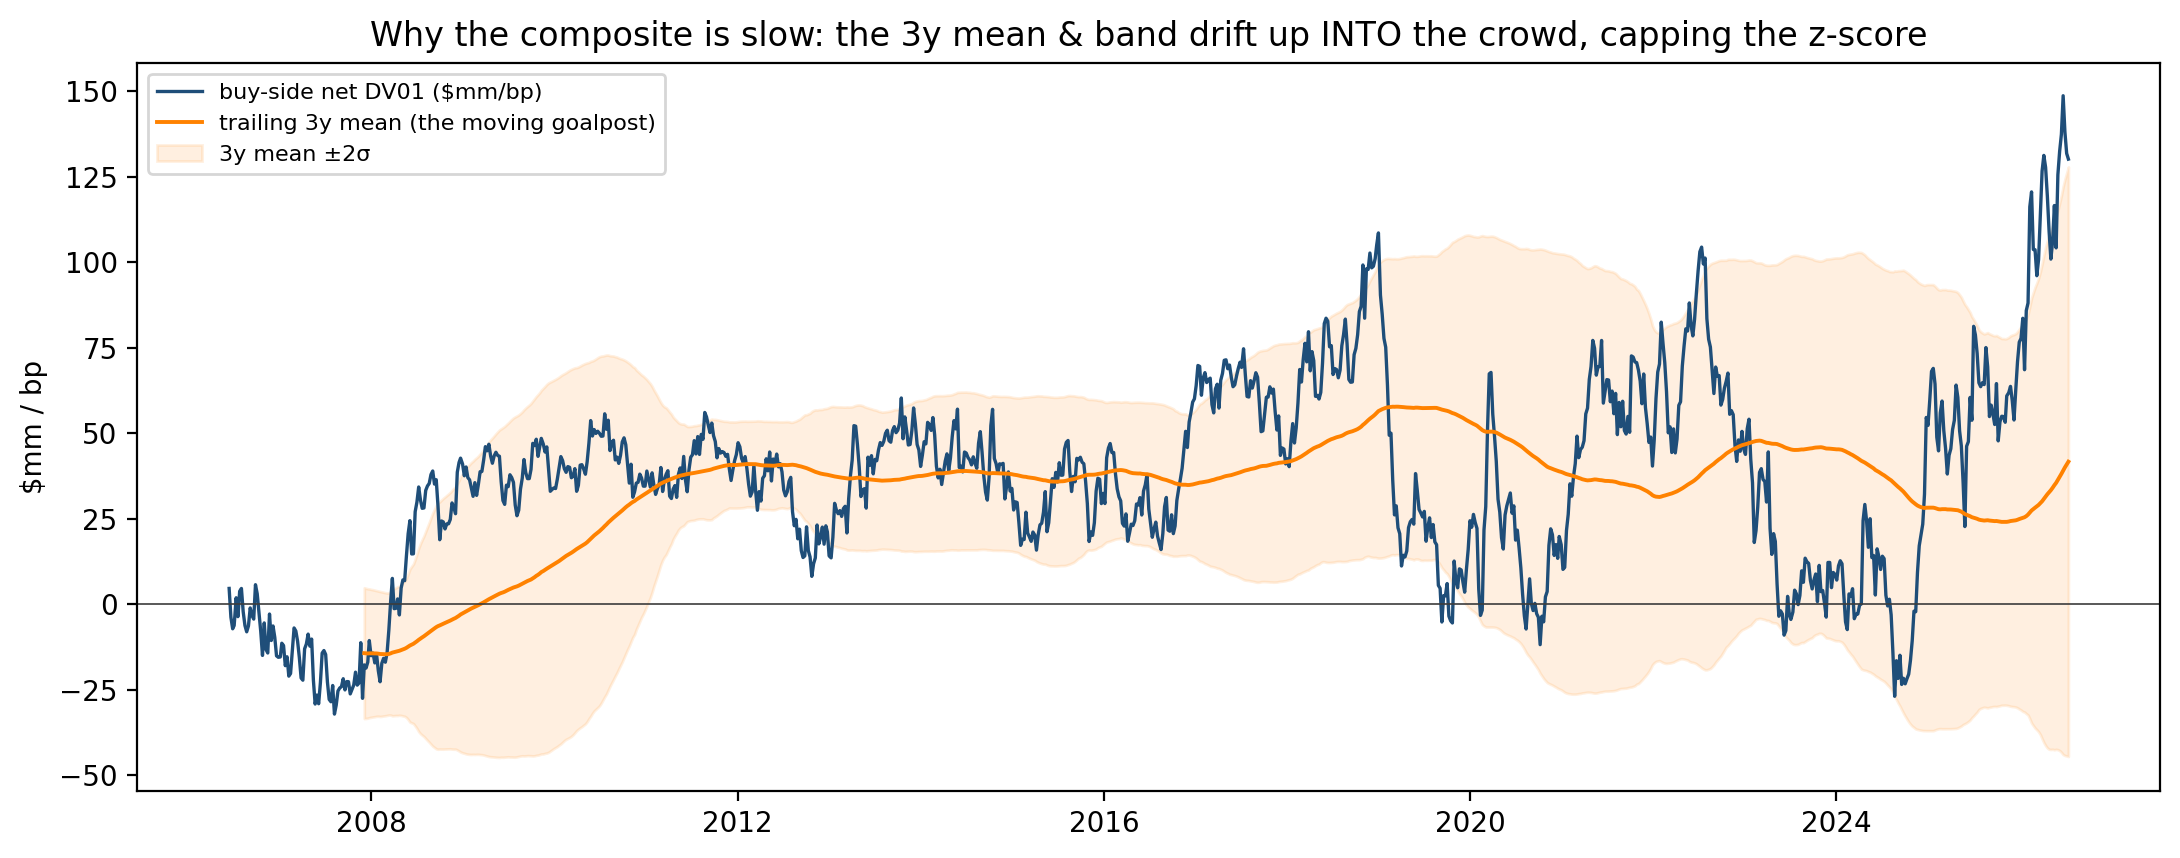
\includegraphics[width=0.92\textwidth]{fig_selfcatchup.png}
\caption*{\footnotesize\textbf{Fig 1.} The 3y mean ($\pm2\sigma$ band) drifts up into the rising position
stock, capping the z-score --- the mechanical source of the lag.}\end{figure}

\subsect{2.2 The double z-score adds a second lag}
Features are 3y-z-scored, PCA-combined, then PC1 is 3y-z-scored \emph{again}. Two passes of 3-year
normalization compound the smoothing. Isolating it: a single-pass 3y-z of the same signal flags the
current crowding roughly \textbf{7 months earlier} than the production (double-pass) composite.

\subsect{2.3 Responsiveness: lead time to flag the current episode}
Applying different normalizations to the \emph{same} buy-side net-DV01 signal and asking when each first
crossed ``crowded'' during the 2024--26 build-up:

\begin{center}\begin{tabular}{lccc}
\toprule
Normalization (same signal) & first ``crowded'' flag & lead vs production & latest reading\\
\midrule
\textbf{Production composite} (2$\times$ 3y-z $+$ PCA) & 2026-01-20 & --- & $z=+2.49$ (near cap)\\
Single-pass 3y-z & 2025-07-01 & $+$29 wks ($\sim$7m) & $z=+2.05$\\
COT-index, 3y (0--100) & 2025-07-01 & $+$29 wks & $89.4$\\
1-year z & 2024-12-17 & $+$57 wks ($\sim$13m) & $z=+1.39$\\
Net-\% -of-OI, 1y z & 2024-12-17 & $+$57 wks & $z=+1.48$\\
EWMA z (half-life 26w) & 2024-12-24 & $+$56 wks & $z=+1.14$\\
COT-index, 1y (0--100) & 2024-12-03 & $+$59 wks & $81.6$\\
Percentile, 1y (0--100) & 2024-06-11 & $+$84 wks & $86.5$\\
Flow (13w change) 1y z & 2024-11-19 & $+$61 wks & $z=-0.64$\\
\bottomrule
\end{tabular}\end{center}

\textbf{The lag is $\sim$13 months.} 1-year-based normalizations flagged this crowding in Nov--Dec 2024;
the production composite waited until Jan 2026. The tell-tale signature of a laggy signal: the fast
metrics have already \emph{peaked and are rolling off} (1y-z $+1.39$, EWMA $+1.14$) while the slow
composite is only now printing its high ($+2.49$) --- it is a rear-view mirror. The flow metric is
already \emph{negative} ($-0.64$): the buy-side stopped adding months ago, which is precisely why the
composite is topping out late.

\begin{figure}[H]\centering
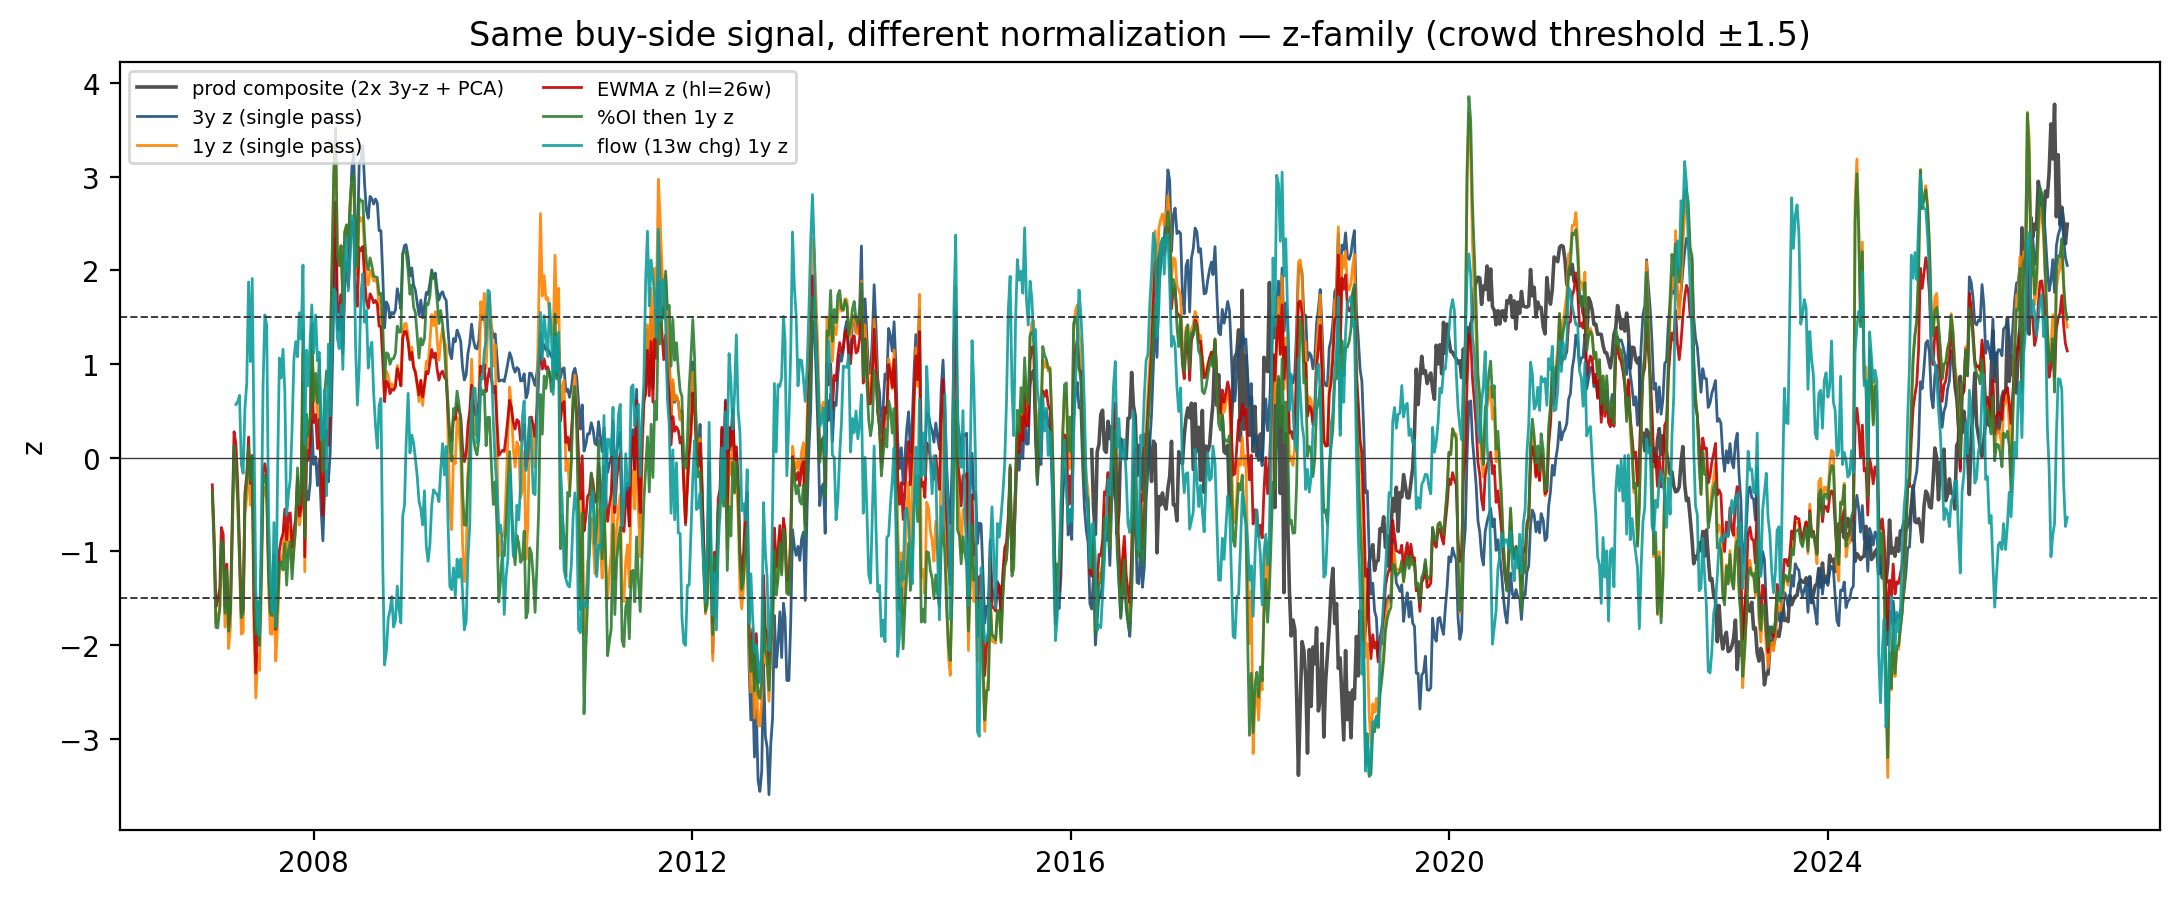
\includegraphics[width=0.49\textwidth]{fig_variants_z.png}\hfill
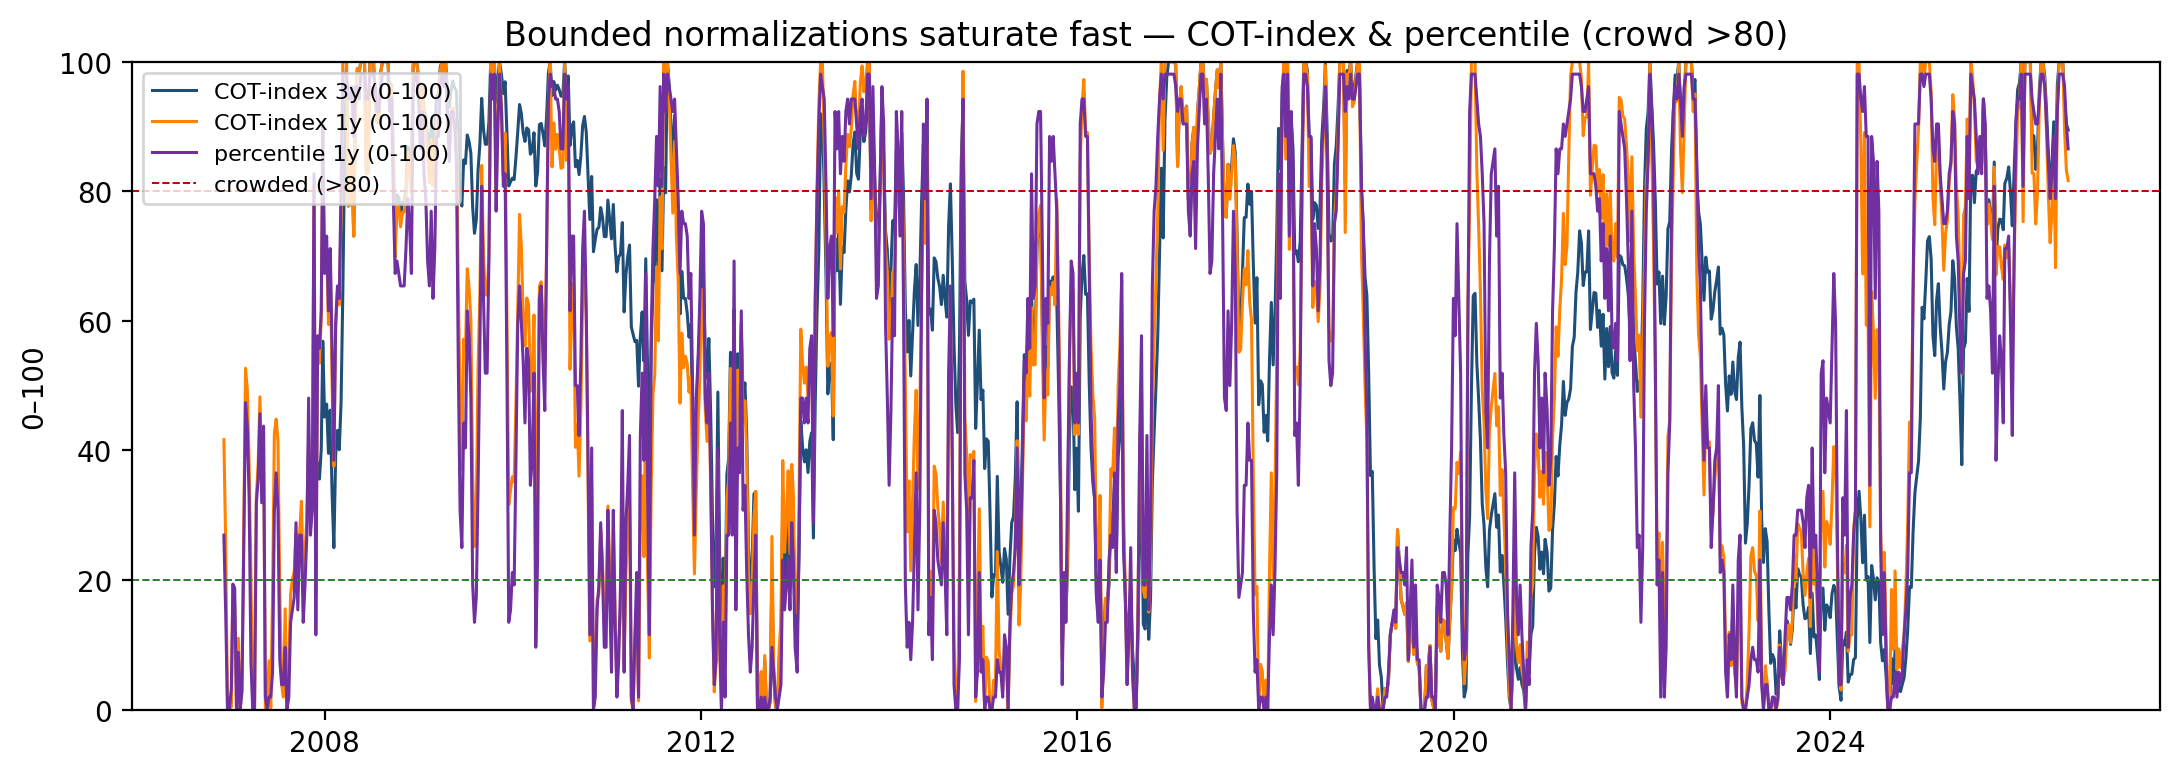
\includegraphics[width=0.49\textwidth]{fig_variants_bounded.png}
\caption*{\footnotesize\textbf{Fig 2.} Same signal, different normalization. Left: z-family (crowd $\pm1.5$)
--- 1y/EWMA lead the 3y composite and turn earlier. Right: bounded COT-index / percentile (crowd $>$80)
--- saturate fast but cannot rank ``crowded vs extremely crowded''.}\end{figure}

\sect{3. How Jefferies and the rest of the Street measure positioning (cited)}
\textbf{Direct answer on Jefferies:} we found \emph{no} public Jefferies CFTC-positioning framework ---
their rates names (Markowska, Simons) are macro/rates economists, not a quant positioning-index desk. The
same is true of TD and RBC. Where banks publish a \emph{rates} positioning gauge it is a \textbf{survey}
(JPMorgan Treasury Client Survey net long$-$short \% \rf{14}; BofA Fund Manager Survey net OW/UW bonds),
not a statistical z-score. Statistical positioning z-scores/percentiles that \emph{are} documented
(Goldman, Deutsche, Nomura) are equity/multi-asset-led and gate their base periods. So the honest
comparison set is the public CFTC/COT methodology and the official-sector (OFR/Fed/TBAC) work.

\begin{center}\begin{tabular}{p{3.1cm}p{3.3cm}cccp{3.2cm}}
\toprule
Source & Normalization & Lookback & Bounded & Lvl/Flow & vs.\ our tool\\
\midrule
\textbf{Modal COT Index} (Barchart, COT Unchained) \rf{1,2} & min-max $(x-\min)/(\max-\min)$ & 3y (also 1y) & 0--100 & Level & bounded, faster; no DV01/PCA\\
\textbf{COT z-score} (COTInsight) \rf{3} & $(x-\mu)/\sigma$ & \textbf{52w} standard & no & Level & \emph{our normalization, but 1/3 our window}\\
Larry Williams (WillCo) \rf{15} & min-max of \textbf{net$\div$OI} & 26w & 0--100 & Level & OI-normalized, very fast\\
\textbf{OFR Hedge Fund Monitor} \rf{7} & \textbf{10y-equiv DV01}, raw \$ & --- & no & Level & \emph{same DV01 idea we use} (best-practice match)\\
CFTC TFF (official) \rf{4} & net, and \textbf{net \% of OI} & --- & --- & Level & we use net; not \%OI\\
US Treasury TBAC \rf{5} & net \% of \textbf{Treasury market} (ex-SOMA) & --- & --- & Level & growth-invariant; we don't do this\\
De Roon et al.\ (JF 2000) \rf{10} & hedging pressure $=$ net$\div$OI & --- & --- & Level & academic \%OI convention\\
SG Trend Indicator (CTA) \rf{13} & 20/120-day MA cross, EWMA vol, vol-target & 3m vol & --- & Flow & positioning as vol-scaled flow, not a level\\
Spectra am/FX \rf{-} & avg of \%OI $+$ 4w-change $+$ skew-z, each rescaled $\pm10$ & mixed & $\pm10$ & Both & bounded multi-source composite\\
Clarus / Litterman-Scheinkman \rf{8} & PCA; \textbf{PC2 $=$ slope} & --- & no & Level & \emph{we already use PCA (PC1/PC2)}\\
CME DV01-neutral 2s10s \rf{9} & size legs so DV01$_1=-$DV01$_2$ & --- & --- & Level & our curve $=$ front$-$long DV01 (same spirit)\\
\bottomrule
\end{tabular}\end{center}

\textbf{Where our tool already leads the mode.} The modal COT Index is a single-contract, level, min-max
index with \emph{no} risk-weighting. Our composite is \emph{more} sophisticated on aggregation: it
DV01-weights across tenors (matching the OFR's canonical 10y-equivalent method \rf{7}) and uses PCA to
de-collinearize (matching the Litterman-Scheinkman / Clarus factor approach \rf{8}). \textbf{Where it
lags the mode:} normalization. The Street's default lookback is 52 weeks (COTInsight explicitly warns 3y
``reacts too slowly to structural shifts'' \rf{3}); many use bounded min-max; the sophisticated add
\emph{flow} (SG's trend model \rf{13}; the academic change-premium \rf{11}) and \emph{\%OI / market-size}
normalization (CFTC \rf{4}, TBAC \rf{5}, De Roon \rf{10}). We do the opposite: a 3-year window applied
twice, on the level only.

\textbf{Context (well sourced).} The asset-manager-long / leveraged-fund-short split we report is the
structure TBAC documents (AM synthetic-duration longs vs LF cash-futures basis shorts, $\sim$92\% $R^2$
since 2015) \rf{5}; the LF Treasury-futures short reached $\sim$\$0.7--1.1tn in 2023--24 per three Fed
FEDS Notes and CFTC staff \rf{6} --- a reminder that a ``crowded'' TFF reading blends the basis trade with
outright macro shorts.

\sect{4. Curve (steepener/flattener) positioning --- methodology and alternatives}
\textbf{Current:} \code{curve\_duration} $=$ front (TU$+$FV) $-$ long (US$+$UB) net DV01, per category,
then the same 3y double-z. This shares the CME DV01-spirit \rf{9} and is a coarse version of PCA-PC2
\rf{8}, but inherits the same 3y lag \emph{and} a level-vs-book ambiguity we already flagged: the current
$z=+1.46$ (lev funds) reads ``crowded steepener'' only relative to a 3y window dominated by a prior
flattener book; the \textbf{raw} front$-$long DV01 is $\approx$ flat ($-0.1$ / $-5.0$ \$mm/bp). Figure~3
separates the two dimensions: \textbf{book tilt} (raw, currently $\approx$0) vs \textbf{positioning
momentum} (the $z$, steepener-direction). Better public templates: OFR 10y-equivalents \rf{7}, PCA PC2
loadings \rf{8}, and a 52w/EWMA or COT-index normalization instead of 3y.

\begin{figure}[H]\centering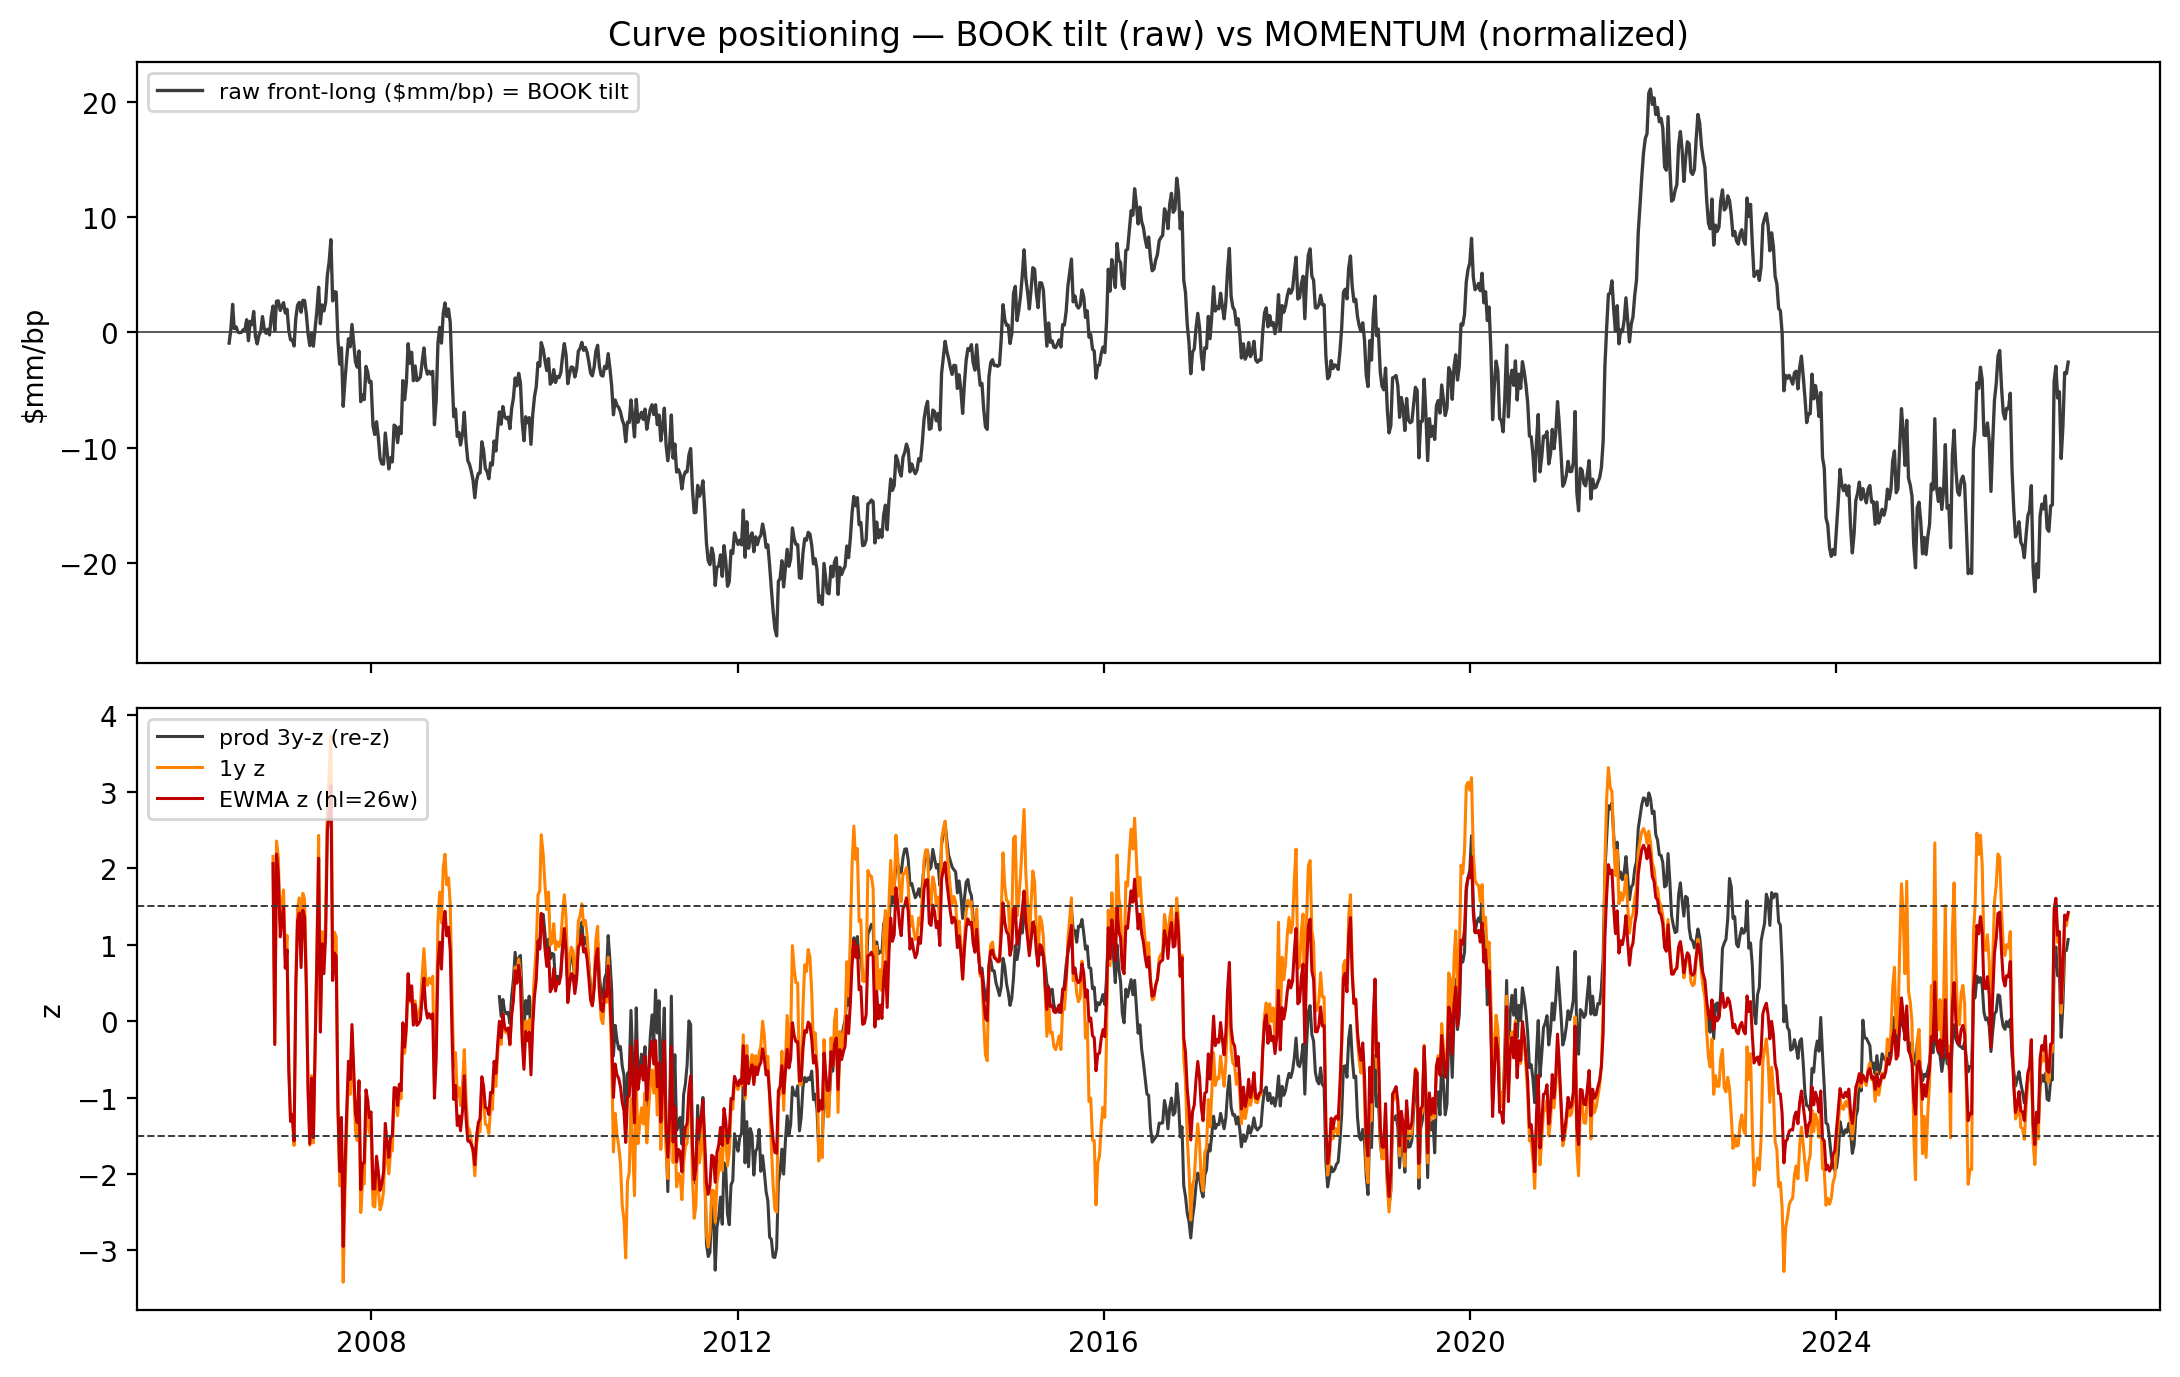
\includegraphics[width=0.92\textwidth]{fig_curve_variants.png}
\caption*{\footnotesize\textbf{Fig 3.} Curve positioning as two distinct things: raw book tilt (top,
$\approx$ flat now) vs normalized momentum (bottom). The production 3y-z is the slowest line.}\end{figure}

\sect{5. Recommendation}
Keep what already matches best practice --- \textbf{DV01 weighting and PCA} (OFR / Litterman-Scheinkman).
Fix the normalization, which is where the tool is slow and where the Street is faster:
\begin{enumerate}[leftmargin=1.4em,itemsep=1pt]
\item \textbf{Shorten \& drop the double-z.} Standardize \emph{once}, over $\sim$52 weeks (or an
\textbf{EWMA} mean/vol, half-life $\sim$26w \rf{3,12}). On the current episode this alone would have
flagged crowding $\sim$7--13 months earlier.
\item \textbf{Normalize by open interest / market size} \rf{4,5,10} so the score is crowding, not a
bigger Treasury market.
\item \textbf{Surface FLOW alongside level} \rf{11,13} --- the 13-week change already turned negative
here, a leading tell the level-z buried.
\item \textbf{Report a bounded COT-index / percentile as a secondary read} \rf{1,2} for an easy
0--100 crowd gauge --- accepting that it saturates (cannot rank crowded vs extremely crowded), so pair it
with the (single-pass) z for magnitude.
\item \textbf{Curve: split book-tilt (raw DV01) from momentum (normalized)} and label them separately;
consider PCA-PC2 \rf{8}.
\end{enumerate}
Keep the 3-year z as a slow ``structural context'' band, not the headline. Net effect: a signal that
reaches over-crowding on the Street's timeline (weeks, not a year late) while retaining the tool's
risk-unit and factor sophistication. \emph{The production default is unchanged in this note; the
alternatives are computed side by side in} \code{results\_positioning\_method/}.

\vspace{4pt}
{\footnotesize\color{biggrey}\textbf{Sources.}
\rf{1} COT Unchained, CoT Index (formula, 3y default, saturation): \url{https://cotunchained.com/en/Info/Commitments-of-Traders-CoT-Reports/CoT-Index}.
\rf{2} Barchart, COT Index (3y, 0--100): \url{https://www.barchart.com/education/technical-indicators/cot-index}.
\rf{3} COTInsight, COT z-score \& window trade-off (52w; ``3y too slow''): \url{https://cotinsight.com/blog/cot-z-score-explained}.
\rf{4} CFTC, TFF Explanatory Notes \& \% of open interest: \url{https://www.cftc.gov/MarketReports/CommitmentsofTraders/ExplanatoryNotes/index.htm}.
\rf{5} US Treasury TBAC, Q1-2024 (AM-long/LF-short, market-size normalization): \url{https://home.treasury.gov/system/files/221/TBACCharge1Q12024.pdf}.
\rf{6} Federal Reserve FEDS Note, hedge-fund Treasury futures/repo (30 Aug 2023): \url{https://www.federalreserve.gov/econres/notes/feds-notes/recent-developments-in-hedge-funds-treasury-futures-and-repo-positions-20230830.html}.
\rf{7} OFR Hedge Fund Monitor, 10-year-equivalent DV01 method: \url{https://www.financialresearch.gov/hedge-fund-monitor/datasets/tff/}.
\rf{8} Clarus FT, PCA of the swap curve (PC2 $=$ slope); Litterman \& Scheinkman (1991): \url{https://www.clarusft.com/principal-component-analysis-of-the-swap-curve-an-introduction/}.
\rf{9} CME, DV01-neutral yield-curve spreads: \url{https://www.cmegroup.com/education/files/yield-curve-spread-trades.pdf}.
\rf{10} De Roon, Nijman \& Veld, hedging pressure $=$ net$\div$OI, J.\ Finance (2000): \url{https://onlinelibrary.wiley.com/doi/10.1111/0022-1082.00253}.
\rf{11} Kang, Rouwenhorst \& Tang, position \emph{changes} vs levels: \url{https://papers.ssrn.com/sol3/papers.cfm?abstract_id=2449315}.
\rf{12} EWMA responsiveness (RiskMetrics $\lambda$; Boyd et al.): \url{https://web.stanford.edu/~boyd/papers/pdf/ewmm.pdf}.
\rf{13} SG Trend Indicator methodology (CTA replica): \url{https://wholesale.banking.societegenerale.com/fileadmin/indices_feeds/SG_Trend_Indicator_Methodology_Summary.pdf}.
\rf{14} JPMorgan Treasury Client Survey (secondary paraphrase): \url{https://uk.investing.com/news/economy-news/treasury-note-investor-sentiment-improves-jpmorgan-poll-shows-93CH-4719315}.
\rf{15} Larry Williams / WillCo min-max lineage (net$\div$OI, 26w): \url{https://cotunchained.com/en/Info/Commitments-of-Traders-CoT-Reports/Williams-Commercial-Index}.
Confidence: \rf{1--13} primary/vendor-methodology or journal; \rf{14} and all bank \emph{rates} indices are secondary paraphrase (no house publishes a rates z-score window). No Jefferies/TD/RBC public CFTC framework was found. The Williams$\to$COT-Index link is algebraic lineage, not a sourced derivation.}
\end{document}
